\begin{figure}[t]
\centering
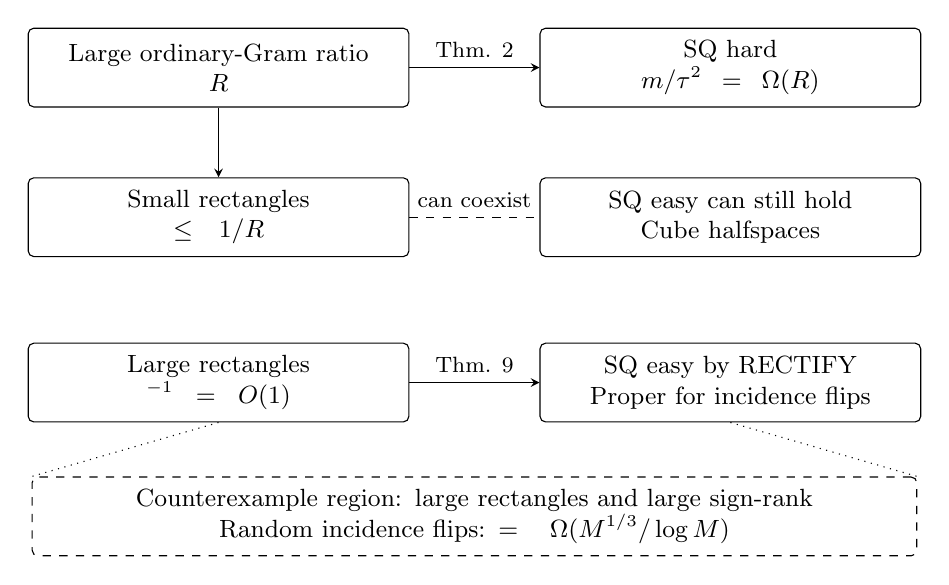
\begin{tikzpicture}[>=stealth,box/.style={draw,rounded corners=2pt,align=center,text width=4.6cm,minimum height=1cm,font=\small},every node/.style={font=\small}]
\node[box] (gram) at (0,3.7) {Large ordinary-Gram ratio\\$R$};
\node[box] (hard) at (6.5,3.7) {SQ hard\\$m/\tau^2=\Omega(R)$};
\node[box] (small) at (0,1.8) {Small rectangles\\$\rect\le1/R$};
\node[box] (half) at (6.5,1.8) {SQ easy can still hold\\Cube halfspaces};
\node[box] (large) at (0,-.3) {Large rectangles\\$\rect^{-1}=O(1)$};
\node[box] (easy) at (6.5,-.3) {SQ easy by RECTIFY\\Proper for incidence flips};
\node[draw,dashed,rounded corners=2pt,align=center,text width=11cm,minimum height=1cm] (sep) at (3.25,-2) {Counterexample region: large rectangles and large sign-rank\\Random incidence flips: $\dc=\Omega(M^{1/3}/\log M)$};
\draw[->] (gram)--node[above,font=\footnotesize]{Thm. 2}(hard);
\draw[->] (gram)--(small);
\draw[dashed] (small)--node[above,font=\footnotesize]{can coexist}(half);
\draw[->] (large)--node[above,font=\footnotesize]{Thm. 9}(easy);
\draw[dotted] (large.south)--(sep.north west);
\draw[dotted] (easy.south)--(sep.north east);
\end{tikzpicture}
\caption{The valid implications and compatible examples. There is no arrow from small rectangles to SQ hardness. A fixed-marginal spectral certificate implies both conclusions separately. The dotted connections locate an example, rather than claim that large rectangles force large sign-rank.}
\label{fig:landscape}
\end{figure}
